% chapters/chapter3/section5.tex
% این فایل توسط main فصل وارد می‌شود، پس نباید \section داشته باشد.

\subsection{همکاری میان تیم توسعه و عملیات}
\label{subsec:ch3-5-collaboration}

\lr{DevOps} تنها مجموعه‌ای از ابزارها و فرایندهای فنی نیست، بلکه یک تغییر فرهنگی و سازمانی عمیق در نحوه‌ی همکاری میان تیم‌های توسعه (\lr{Development}) و عملیات (\lr{Operations}) است. این فرهنگ بر پایه‌ی اعتماد، ارتباط، شفافیت و مسئولیت مشترک بنا شده است. بر اساس پژوهش \cite{Jha2023}، \lr{DevOps} پیش از آن‌که رویکردی فنی باشد، نوعی تغییر در نگرش سازمانی است که موجب نزدیکی میان تیم‌های مختلف و شکل‌گیری ذهنیت همکاری می‌شود.

در مدل‌های سنتی، توسعه‌دهندگان پس از نوشتن کد، آن را تحویل تیم عملیات می‌دادند تا در محیط واقعی مستقر شود. نتیجه‌ی این جدایی، بروز مشکلاتی مانند عدم هماهنگی، خطاهای زیاد در استقرار و تأخیر در تحویل بود. \lr{DevOps} با هدف رفع این شکاف به‌وجود آمد تا توسعه و عملیات به‌صورت یک واحد عمل کنند و مسئولیت موفقیت یا شکست نرم‌افزار را به‌صورت مشترک بر عهده بگیرند.

\subsection{مؤلفه‌های اصلی فرهنگ \lr{DevOps}}
\label{subsec:ch3-5-components}

\textbf{ارتباط باز و مداوم:} تیم‌ها باید به‌طور پیوسته با یکدیگر در ارتباط باشند. ابزارهایی مانند \lr{Slack} یا \lr{Microsoft Teams} برای گفت‌وگوهای لحظه‌ای، و \lr{Jira} برای پیگیری وظایف به‌کار می‌روند. این ارتباط مداوم باعث می‌شود تصمیم‌ها سریع‌تر گرفته شوند و مشکلات پیش از تبدیل‌شدن به بحران، شناسایی و رفع شوند. نمونه‌ی عملی آن در شرکت \lr{Atlassian} دیده می‌شود که توسعه‌دهندگان و مدیران سیستم وضعیت پایپ‌لاین‌های \lr{CI/CD} و استقرارها را در همان کانال‌های گفت‌وگو دنبال می‌کنند.

\textbf{مسئولیت مشترک (\lr{Shared Ownership}):} در فرهنگ \lr{DevOps} دیگر مفهوم «تحویل دادن کد و رها کردن آن» وجود ندارد. توسعه‌دهندگان در موفقیت نرم‌افزار پس از استقرار نیز نقش مستقیم دارند و در مقابل، تیم عملیات هم از مراحل طراحی و تست در جریان پروژه قرار می‌گیرد. مثال شناخته‌شده، سیاست «\lr{You build it, you run it}» در شرکت \lr{Amazon} است که باعث می‌شود توسعه‌دهنده نسبت به پایداری و مانیتورینگ نرم‌افزار در محیط واقعی حساس‌تر باشد.

\textbf{یادگیری و بهبود مستمر (\lr{Continuous Learning}):} پس از هر انتشار (\lr{Release})، تیم‌ها جلساتی با عنوان \lr{Postmortem} برگزار می‌کنند تا شکست‌ها و موفقیت‌ها را بررسی کنند. هدف، سرزنش افراد نیست؛ بلکه یافتن علت ریشه‌ای خطا و اصلاح فرایند است. شرکت‌هایی مانند \lr{Google} از گزارش‌های \lr{Blameless Postmortem} استفاده می‌کنند تا بدون مقصر جلوه‌دادن افراد، فرایندها و پیکربندی‌ها را بهبود دهند.

\textbf{هم‌ترازی اهداف بین تیم‌ها (\lr{Goal Alignment}):} در سازمان‌های سنتی، اهداف توسعه (تحویل سریع‌تر) و عملیات (پایداری بیشتر) معمولاً در تضاد هستند. \lr{DevOps} با تعریف شاخص‌های عملکرد مشترک مانند \lr{MTTR} و \lr{Deployment Frequency} این تضاد را کاهش می‌دهد و باعث می‌شود هر دو تیم به سمت هدف مشترک، یعنی تحویل سریع ولی پایدار نرم‌افزار، حرکت کنند. همان‌طور که در \cite{Jha2023} آمده است، هم‌ترازی هدف‌ها باعث می‌شود معیارهای ارزیابی از فردمحور به تیم‌محور تغییر کند.

\begin{figure}[H]
    \centering
    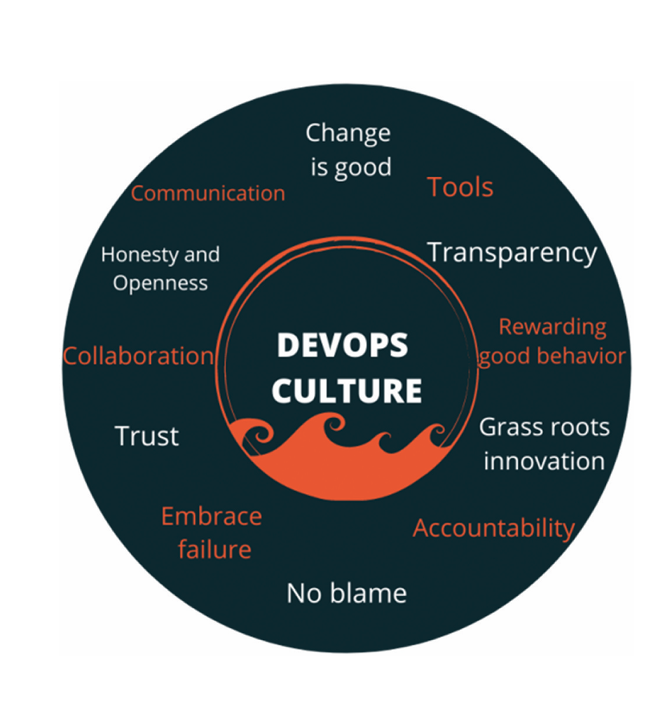
\includegraphics[width=0.8\textwidth]{devops-culture.png}
    \caption{نمایی از مؤلفه‌های فرهنگ و ذهنیت \lr{DevOps} بر اساس \cite{Jha2023}.}
    \label{fig:devops-culture}
\end{figure}
